\chapter{Regroupement Modulaire}

Dans la \autoref{fig:25-regroupement_modulaire}, nous pouvons identifier les multiples parties composant notre application.

\begin{figure}[h]
    \centering
    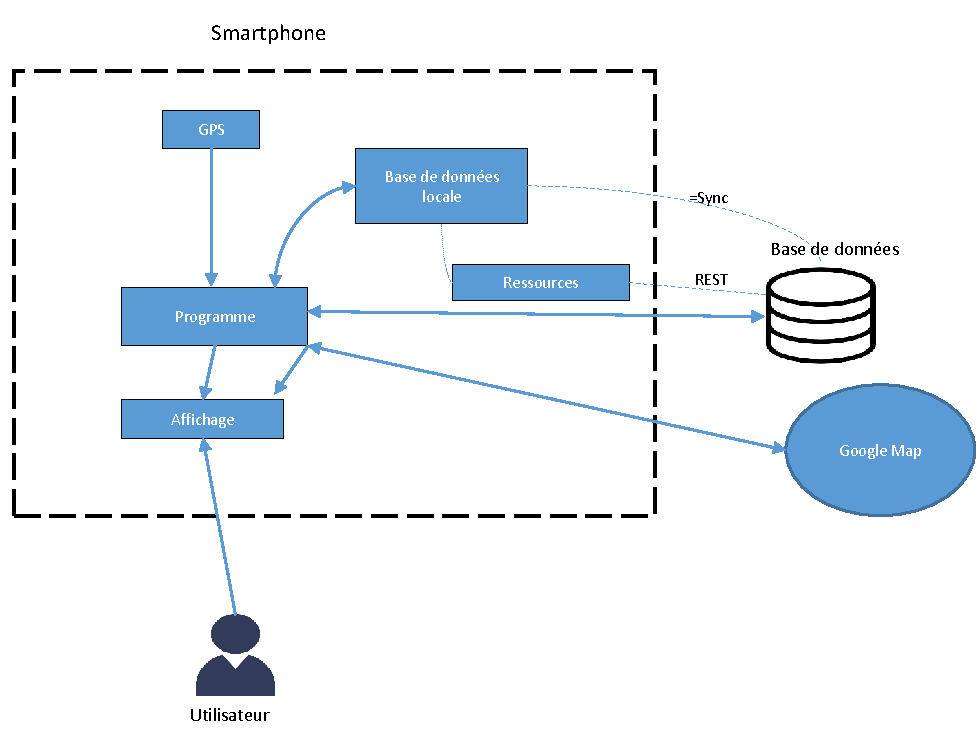
\includegraphics[keepaspectratio, width=2\textwidth/2, height=2\textheight/5]{ima/regroupement_modulaire}
    \caption{Schéma fonctionnel de notre projet.}
    \label{fig:25-regroupement_modulaire}
\end{figure}

\section{GPS}

% Expliquer ce que c'est, ce pourquoi l'appli s'en sert et à quelle fréquence, etc.

\section{Base de données}

\section{Google Maps}

\section{Resources externes}

\section{Affichage}
